\documentclass[12pt, letterpaper]{article}
\usepackage{graphicx}
\graphicspath{.}
\title{My test doc}
\author{Kevin Zhang}
\date{Nov 2023}
\begin{document}
\maketitle
First document. This is a \textbf{simple} example, with \textbf{\textit{no 
extra parameters}} or \underline{packages included}.

Some of the greatest \emph{discoveries} in science 
were made by accident.

\textit{Some of the greatest \emph{discoveries} 
in science were made by accident.}

\textbf{Some of the greatest \emph{discoveries} 
in science were made by accident.}
% thie is a comment line.

% The \includegraphcs command is provided (implemented) by the 
% graphicx package
\begin{figure}[h]
	\centering
	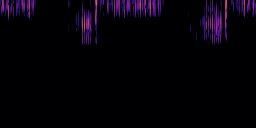
\includegraphics[width=0.75\textwidth]{mix_7_s1.png} 
	\caption{mix 7 s1}
	\label{fig:sound1}
\end{figure}

\textbf{Unordered list}
\begin{itemize}
	\item The individual entries are indicated with a black dot, a so-called bullet.
	\item The text in the entries may be of any length.
\end{itemize}
\textbf{Ordered list}
\begin{enumerate}
	\item This is the first entry in our list.
	\item The list numbers increase with each entry we add.
\end{enumerate}
\textbf{Inline math mode\\}
In physics, the mass-energy equivalence is stated 
by the equation $E=mc^2$, discovered in 1905 by Albert Einstein.
\textbf{\\Display math mode\\}
The mass-energy equivalence is described by the famous equation
\[ E=mc^2 \] discovered in 1905 by Albert Einstein. 

In natural units ($c = 1$), the formula expresses the identity
\begin{equation}
E=m
\end{equation}
\end{document}
